\section{Многолучевая интерференция. Интерферометр Фабри-Перо}

\begin{figure}[H]
	\centering
	\begin{tikzpicture}[scale=1.2]
		% Зеркала
		\draw[thick, fill=blue!10] (1,-2) rectangle (1.2,2);
		\draw[thick, fill=blue!10] (3,-2) rectangle (3.2,2);
		
		\node[above] at (1.1, 2) {$R \sim 99.8\%$};
		\node[below] at (2.1, -2.2) {$d$};
		\draw[<->] (1.2, -2) -- (3, -2);
		
		% Падающий луч
		\draw[thick, blue, ->] (-1, 1.5) -- (1, 0.5) node[midway, above left] {$E_0$};
		\draw[dashed, blue] (-1, 0.5) -- (1, 0.5);
		\draw[blue] (-0.3, 0.5) arc (180:153:0.7) node[midway, left] {$\alpha$};
		
		% Отраженные лучи
		\draw[thick, blue, ->] (1, 0.5) -- (-1, -0.5) node[midway, below right] {$rt E_0$};
		
		% Внутри и на выходе
		\draw[thick, blue, ->] (1, 0.5) -- (3, -0.5); % t E_0
		\node[above right] at (1, 0.5) {$t E_0$};
		
		\draw[thick, blue, ->] (3, -0.5) -- (5, -1.5) node[right] {$E_0 t^2$};
		\node[right] at (3, -0.5) {$t$};
		\node[left] at (1, 0.5) {$r, t$};
		
		\draw[thick, blue, ->] (3, -0.5) -- (1, -1.5) node[midway, above] {$t E_0 r$};
		\draw[thick, blue, ->] (1, -1.5) -- (3, -2.5);
		\draw[thick, blue, ->] (3, -2.5) -- (5, -3.5) node[right] {$E_0 t^2 r^2 e^{i \delta \varphi}$};
		
		\node[text width=2cm, align=center] at (-1.5, 0) {\small коэфф. отраж.};
		\node[text width=2cm, align=center] at (-1.5, -1) {\small коэфф. пропуск.};
	\end{tikzpicture}
\end{figure}

Сложим амплитуды прошедших лучей:
\begin{align*}
	E &= E_0 t^2 \qty(1 + r^2 e^{i \delta \varphi} + r^4 e^{2i \delta \varphi} + \dots) = \frac{E_0 t^2}{1 - r^2 e^{i \delta \varphi}} \\
	I &= |E|^2 = E E^* = \frac{E_0 t^2}{1 - r^2 e^{i \delta \varphi}} \cdot \frac{E_0 t^2}{1 - r^2 e^{-i \delta \varphi}} = \frac{E_0^2 t^4}{1 + r^4 - 2r^2 \cos \delta \varphi} = \\
	&= \left\{ 1 + r^4 - 2r^2 \cos \delta \varphi + 2r^2 - 2r^2 = (1 - r^2)^2 + 2r^2 (1 - \cos \delta \varphi) = (1 - R)^2 + 4R \sin^2 \frac{\delta \varphi}{2} \right\} \\
	&= \frac{I_0 (1 - R)^2}{(1 - R)^2 + 4R \sin^2 \frac{\delta \varphi}{2}} = \frac{I_0}{1 + \frac{4R}{(1 - R)^2} \sin^2 \frac{\delta \varphi}{2}}, \quad R \to 1 \quad \begin{cases} 0 \\ I_0, \, \sin \frac{\delta \varphi}{2} = 0 \Rightarrow \frac{\delta \varphi}{2} = \pi m \end{cases}
\end{align*}

Условие максимума:
\begin{equation}
	\frac{k \Delta}{2} = \pi m \implies \frac{2\pi}{\lambda} \cdot \frac{nd \cos \alpha}{2} = \pi m
\end{equation}

\begin{itemize}
	\item \textbf{Минимальное значение интенсивности:}
	$$I_{\min} = \frac{I_0}{1 + \frac{4R}{(1 - R)^2}} = \frac{I_0 (1 - R)^2}{1 - 2R + R^2 + 4R} = \frac{I_0 (1 - R)^2}{(1 + R)^2}$$
	\item \textbf{Резкость:}
	$$\frac{I_{\max}}{I_{\min}} = \frac{(1 + R)^2}{(1 - R)^2} \xrightarrow{R \to 1} \infty$$
\end{itemize}

\begin{figure}[H]
	\centering
	\begin{tikzpicture}
		\draw[->] (-0.5, 0) -- (8, 0) node[right] {$\delta \varphi$};
		\draw[->] (0, -0.5) -- (0, 3) node[above] {$I$};
		
		\draw[thick, blue, samples=200, domain=0:7.5] plot (\x, {2.5/(1 + 0.5*(sin(\x*180/3.1415*2))^2)});
		\draw[thick, red, samples=300, domain=0:7.5] plot (\x, {2.5/(1 + 20*(sin(\x*180/3.1415*2))^2)});
		\draw[thick, black, samples=400, domain=0:7.5] plot (\x, {2.5/(1 + 200*(sin(\x*180/3.1415*2))^2)});
		
		\node[blue] at (1.5, 1.5) {$R = 0.3$};
		\node[red] at (2.5, 0.8) {$R = 0.5$};
		\node[black] at (3.5, 0.4) {$R \to 1$};
		\node[right] at (5, 1.5) {$R$ очень малое};
		\draw[->] (5, 1.5) -- (3.3, 0.5);
		
		\node[below] at (1.57, 0) {$2\pi m$};
		\node[below] at (3.14, 0) {$2\pi (m+1)$};
		\node[below] at (4.71, 0) {$2\pi (m+2)$};
		
		\draw[<->, red] (1.3, 1.25) -- (1.84, 1.25) node[midway, above] {$\varepsilon$};
	\end{tikzpicture}
\end{figure}

Ширина пика $\varepsilon$:
$$I(\varepsilon) = \frac{1}{2} I_{\max}$$
$$\frac{I_0}{1 + \frac{4R}{(1 - R)^2} \sin^2 \frac{\varepsilon}{4}} = \frac{I_0}{2} \implies \sin \frac{\varepsilon}{4} = \frac{(1 - R)}{\sqrt{R}} \xrightarrow{R \to 1} 0$$

\section{Дифракция}

\begin{definition}{Дифракция}{}
	\textbf{Дифракция} — совокупность явлений, наблюдаемых при распространении света в среде с резкими неоднородностями и связанных с отклонениями от законов геометрической оптики. ($\hookrightarrow$ края, отверстия, щели).
\end{definition}

\begin{itemize}
	\item Огибание световыми волнами препятствий.
	\item Проникновение в область геометрической тени (кривизной волнового фронта можно пренебречь).
	\item \textbf{Типы:}
	\begin{enumerate}
		\item Фраунгофера (в параллельных пучках в дальней зоне, дифрагируют плоские волны).
		\item Френеля (в сходящихся пучках в ближней зоне).
	\end{enumerate}
	\item Общая задача дифракции:
\end{itemize}

\begin{figure}[H]
	\centering
	\begin{tikzpicture}
		\draw[->, thick] (-2, 0) -- (-0.5, 0) node[midway, above] {$\vb{E}_0$} node[below] {$\vb{k}_0$};
		\draw[thick, fill=blue!10, decorate, decoration={random steps,segment length=3pt,amplitude=1pt}] (0,-1) rectangle (1,1);
		\node at (0.5, 0) {$n(\vb{r})$};
		\node[above] at (0.5, 1.2) {тело конечных размеров};
		
		\draw[->, thick] (1.5, 0) -- (3, 0) node[midway, above] {$\vb{E}$} node[below] {$\vb{k}$};
		\node[below] at (0.5, -1) {$S(\vb{r})$};
		
		\node at (1.5, -1.8) {$\vb{E}_0 \to \vb{E}_0 + \vb{E}'$};
		\draw[->] (1.5, -2.1) -- (2.2, -1.8);
		\node[below, text width=4cm, align=center] at (2.2, -2.1) {поле, генерируемое телом конечных размеров};
	\end{tikzpicture}
\end{figure}

\subsection{Приближенные методы}

\subsubsection{(1) Принцип Гюйгенса}
\begin{itemize}
	\item Способ геометрического построения волнового фронта.
	\item Каждая точка волнового фронта является центром вторичных сферических волн, радиус каждой сферы опред. скоростью распрост. ЭМ волн в данной области среды.
	\item Волновой фронт в последующие моменты времени является огибающей вторичных волн.
\end{itemize}

\begin{figure}[H]
	\centering
	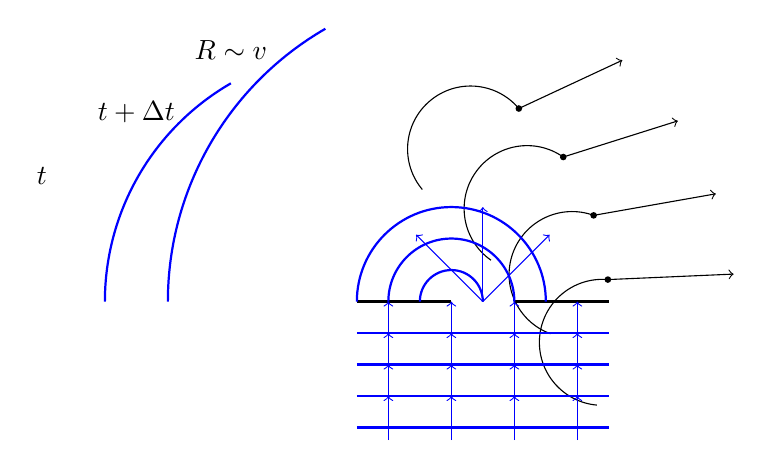
\begin{tikzpicture}[scale=0.8]
		% Левый рисунок
		\draw[thick, blue] (0,0) arc (180:120:4);
		\draw[thick, blue] (1,0) arc (180:120:5);
		
		\foreach \a in {130, 145, 160, 175} {
			\fill ({-4*cos(\a)+4}, {4*sin(\a)}) circle (1.5pt);
			\draw[thin] ({-4*cos(\a)+4}, {4*sin(\a)}) arc (\a-90:\a+90:1);
			\draw[->] ({-4*cos(\a)+4}, {4*sin(\a)}) -- ({-5*cos(\a)+5}, {5*sin(\a)});
		}
		
		\node at (-1, 2) {$t$};
		\node at (0.5, 3) {$t+\Delta t$};
		\node at (2, 4) {$R \sim v$};
		
		% Правый рисунок
		\begin{scope}[xshift=6cm]
			\draw[thick] (-2, 0) -- (-0.5, 0);
			\draw[thick] (0.5, 0) -- (2, 0);
			
			\foreach \y in {-0.5, -1, -1.5, -2} {
				\draw[blue, thick] (-2, \y) -- (2, \y);
				\draw[->, blue] (-1.5, \y-0.2) -- (-1.5, \y+0.5);
				\draw[->, blue] (-0.5, \y-0.2) -- (-0.5, \y+0.5);
				\draw[->, blue] (0.5, \y-0.2) -- (0.5, \y+0.5);
				\draw[->, blue] (1.5, \y-0.2) -- (1.5, \y+0.5);
			}
			
			\draw[blue, thick] (0,0) arc (0:180:0.5);
			\draw[blue, thick] (0.5,0) arc (0:180:1);
			\draw[blue, thick] (1,0) arc (0:180:1.5);
			
			\draw[->, blue] (0,0) -- (0, 1.5);
			\draw[->, blue] (0,0) -- (-1.06, 1.06);
			\draw[->, blue] (0,0) -- (1.06, 1.06);
		\end{scope}
	\end{tikzpicture}
\end{figure}

\subsubsection{(2) Принцип Гюйгенса-Френеля}
Каждый элемент волнового фронта является центром возмущения, порождающим вторичные сферические волны, в результате интерференции которых формируется результирующее световое поле в каждой точке пр-ва, полное световое поле — рез-т интерференции вторичных волн.

\begin{figure}[H]
	\centering
	\begin{tikzpicture}
		\draw[thick, blue] (0, 3) arc (60:-60:3);
		\fill (0.5, 0.5) circle (1.5pt);
		\draw[thick, ->] (0.5, 0.5) -- (1.2, 1.2) node[above] {$d\vb{S}$};
		\draw[thick, ->] (0.5, 0.5) -- (2.5, 0.5) node[midway, below] {$\vb{r}$};
		\fill (2.5, 0.5) circle (1.5pt) node[right] {$P$};
		
		\node[text width=3cm] at (-1.5, 2) {поле, которое создает $dS$ $\sim \frac{E_0}{r} e^{ikr}$};
		\node at (5, 2) {$dE_P \sim \frac{E_0}{r} e^{ikr} \leftarrow$ волновое число};
		\node at (5, 1) {$dE_P = K(\alpha) \frac{E_0}{r} e^{ikr} dS$};
		\node[fill=green!20, rounded corners, inner sep=5pt] at (5, 0) {$E_P = \iint\limits_S K(\alpha) \frac{E_0}{r} e^{ikr} dS$ интеграл Френеля};
		
		\draw[->, dashed] (0.5, 0.5) -- (-1, 0.5);
		\draw[->, dashed] (0.5, 0.5) -- (0.5, -1);
		
		\node[fill=yellow!20, rounded corners, inner sep=3pt] at (6, -1.5) {$K(\alpha_0, \alpha_1) = -\frac{i}{2\lambda} (\cos \alpha_0 + \cos \alpha_1)$ Кирхгоф, $k = \frac{2\pi}{\lambda}$};
	\end{tikzpicture}
\end{figure}

\subsection{Прохождение света через плоский экран}

\begin{figure}[H]
	\centering
	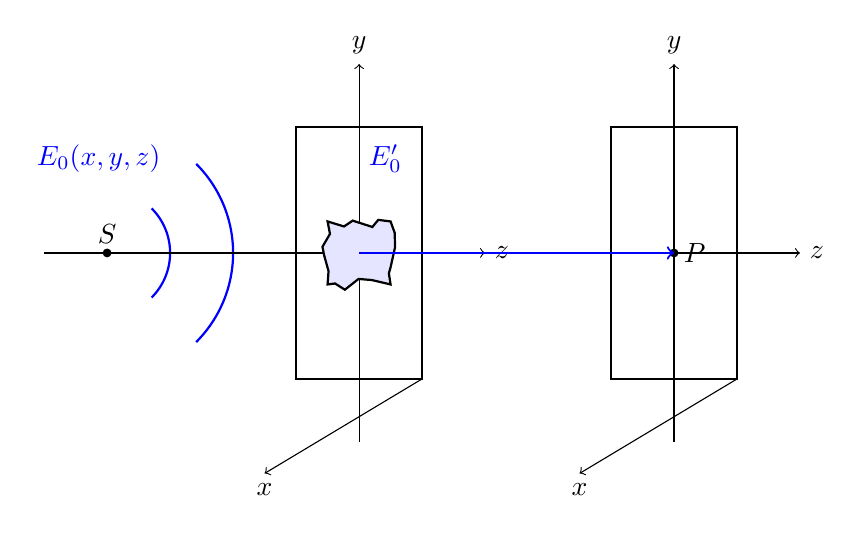
\begin{tikzpicture}[scale=0.8]
		% Источник и сферические волны
		\fill (-4, 1) circle (2pt) node[above] {$S$};
		\draw[blue, thick] (-3, 1) arc (0:45:1);
		\draw[blue, thick] (-3, 1) arc (0:-45:1);
		\draw[blue, thick] (-2, 1) arc (0:45:2);
		\draw[blue, thick] (-2, 1) arc (0:-45:2);
		
		% Экран 1
		\draw[thick] (-1, -1) rectangle (1, 3);
		\draw[->] (0, -2) -- (0, 4) node[above] {$y$};
		\draw[->] (-5, 1) -- (2, 1) node[right] {$z$};
		\draw[->] (1, -1) -- (-1.5, -2.5) node[below] {$x$};
		
		\draw[thick, fill=blue!10, decorate, decoration={random steps,segment length=5pt,amplitude=2pt}] (-0.5, 0.5) rectangle (0.5, 1.5);
		
		% Экран 2
		\begin{scope}[xshift=5cm]
			\draw[thick] (-1, -1) rectangle (1, 3);
			\draw[->] (0, -2) -- (0, 4) node[above] {$y$};
			\draw[->] (-2, 1) -- (2, 1) node[right] {$z$};
			\draw[->] (1, -1) -- (-1.5, -2.5) node[below] {$x$};
			\fill (0, 1) circle (2pt) node[right] {$P$};
		\end{scope}
		
		\draw[blue, thick, ->] (0, 1) -- (5, 1);
		
		\node[left, blue] at (-3, 2.5) {$E_0(x,y,z)$};
		\node[right, blue] at (0, 2.5) {$E'_0$};
	\end{tikzpicture}
\end{figure}

Функция пропускания экрана: 
$$t(x,y) = \begin{cases} 1, & \text{если экрана нет} \\ 0, & \text{если пропуск нет} \end{cases}, \quad 0 < t(x,y) < 1$$
$E_0(x,y,z)$ — перед экраном \\
$E'_0(x,y,z)$ — сразу после экрана \qquad $E'_0(x,y,z) = t(x,y) E_0(x,y,z)$
$$E_P \sim \iint\limits_S \frac{e^{ikr}}{r} E_0(x,y,z) t(x,y) (\cos \alpha_0 + \cos \alpha_1) dx dy$$

\section{Дифракция Френеля на круглом отверстии}

\begin{figure}[H]
	\centering
	\begin{tikzpicture}[scale=0.9]
		\draw[->] (-1, 0) -- (6, 0) node[right] {$z$};
		\draw[->] (0, -2) -- (0, 2) node[above] {$y$};
		\draw[->] (0, 0) -- (-1, -1) node[below] {$x$};
		
		\draw[thick] (0, -1.5) rectangle (0, 1.5);
		\draw[thick, fill=white] (0, 0) circle (0.5);
		
		\fill (-2, 0) circle (2pt) node[below] {$S$};
		\fill (4, 0) circle (2pt) node[below] {$P$};
		
		\draw[blue, ->] (-2, 0) -- (-1, 0.5);
		\draw[blue, ->] (-2, 0) -- (-1, -0.5);
		
		\begin{scope}[xshift=8cm]
			\fill (-2, 0) circle (2pt) node[below] {$S$};
			\fill (4, 0) circle (2pt) node[below] {$P$};
			\draw[->] (-3, 0) -- (5, 0) node[right] {$z$};
			
			\draw[thick, pattern=north east lines] (0, 1) rectangle (0.2, 2.5);
			\draw[thick, pattern=north east lines] (0, -1) rectangle (0.2, -2.5);
			
			\draw[dashed] (-2, 0) -- (0, 1.5) node[midway, above left] {$R$};
			\draw[dashed] (0, 1.5) -- (4, 0) node[midway, above right] {$r$};
			\draw[thick, blue] (-2, 0) -- (0, 1) -- (4, 0);
			
			\draw[blue] (0, 1.5) arc (90:270:1.5 and 0.3);
			\draw[blue, dashed] (0, 1.5) arc (90:-90:1.5 and 0.3);
			
			\node[below] at (2, 0) {$z$};
			\draw[<->] (0, -0.2) -- (4, -0.2);
		\end{scope}
	\end{tikzpicture}
\end{figure}

\begin{align*}
	dS &= 2\pi R \sin \theta R d\theta = 2\pi R^2 \sin \theta d\theta \\
	r^2 &= R^2 + (R+z)^2 - 2R(R+z)\cos\theta \\
	2r dr &= 2R(R+z)\sin\theta d\theta \implies \sin\theta d\theta = \frac{r dr}{R(R+z)} \\
	dS &= 2\pi R^2 \frac{r dr}{R(R+z)} = 2\pi R \frac{r dr}{R+z}
\end{align*}

$$E_P \sim \iint\limits_S E_0 \frac{e^{ikR}}{R} \cdot \frac{e^{ikr}}{r} \cdot K(\alpha) dS$$
$$E_P \sim E_0 \frac{e^{ikR}}{R} \frac{e^{ikr}}{r} \cdot 2\pi \frac{R}{R+z} \int \underbrace{e^{ikr} K(\alpha)}_{\text{быстрая функция}} \underbrace{dr}_{\text{медленная ф-ия}}$$

\begin{figure}[H]
	\centering
	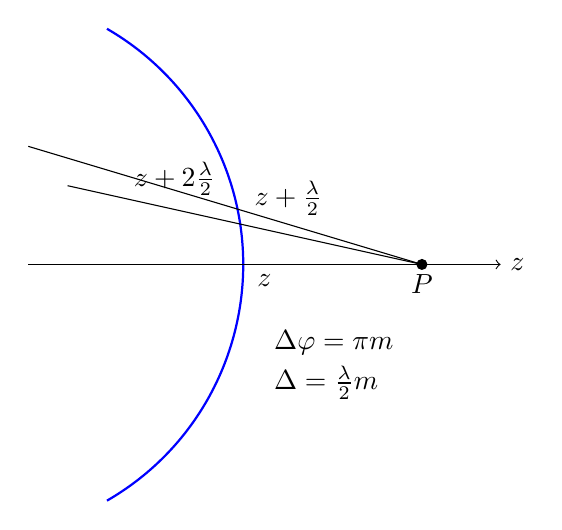
\begin{tikzpicture}
		\draw[->] (-1, 0) -- (5, 0) node[right] {$z$};
		\draw[thick, blue] (0, -3) arc (-60:60:3.46);
		\fill (4, 0) circle (2pt) node[below] {$P$};
		
		\draw (0,0) -- (4,0) node[midway, below] {$z$};
		\draw (-0.5, 1) -- (4,0) node[midway, above right] {$z+\frac{\lambda}{2}$};
		\draw (-1, 1.5) -- (4,0) node[midway, above left] {$z+2\frac{\lambda}{2}$};
		
		\node[right] at (2, -1) {$\Delta \varphi = \pi m$};
		\node[right] at (2, -1.5) {$\Delta = \frac{\lambda}{2} m$};
	\end{tikzpicture}
\end{figure}

\begin{itemize}
	\item Вклад одной зоны:
	$$E_m \sim K_m \int\limits_{z+(m-1)\frac{\lambda}{2}}^{z+m\frac{\lambda}{2}} e^{ikr} dr = \frac{K_m}{ik} e^{ikr} \eval_{z+(m-1)\frac{\lambda}{2}}^{z+\frac{\lambda}{2}m} =$$
	$$= \frac{\lambda K_m}{2\pi i} \qty[ e^{ikz} e^{ikm\frac{\lambda}{2}} - e^{ikz} e^{ik(m-1)\frac{\lambda}{2}} ] = \frac{\lambda K_m}{2\pi i} e^{ikz} \qty[ e^{i\pi m} - e^{i\pi m} e^{-i\pi} ] = $$
	$$= \frac{\lambda K_m}{2\pi i} e^{ikz} e^{i\pi m} \qty[1 - (-1)] = \frac{\lambda K_m}{\pi i} e^{ikz} (-1)^m$$
\end{itemize}

$$E_m = \frac{\lambda K_m}{\pi i} e^{ikz} (-1)^m$$
\begin{align*}
	E_P &\sim E_0 \frac{e^{ikR}}{R} 2\pi \frac{R}{R+z} \sum_{m=1}^{N} \frac{\lambda K_m}{\pi i} (-1)^m e^{ikz} = \frac{2 E_0 \lambda}{i} \frac{e^{ik(R+z)}}{R+z} \sum_{m=1}^{N} K_m (-1)^m = \\
	&= const \cdot E_0 (K_1 - K_2 + K_3 - K_4 + \dots)
\end{align*}
Здесь $E_1 > E_2 > E_3 > \dots$ вклад одной зоны.

\begin{definition}{Зоны Френеля}{fresnel_zones}
	\textbf{Зоны Френеля} — небольшие области волнового фронта, от противоположных границ которых излучение приходит в точку наблюдения, сдвинутым по фазе на $\pi$. Соседние зоны находятся в противофазе.
\end{definition}

\begin{figure}[H]
	\centering
	\begin{tikzpicture}[scale=0.8]
		% Спираль
		\draw[->] (-3, 0) -- (3, 0) node[right] {$\text{Re} E$};
		\draw[->] (0, -1) -- (0, 3) node[above] {$\text{Im} E$};
		\draw[thick, blue, domain=0:25.13, samples=300] plot ({1.5*cos(\x r)*exp(-0.05*\x) + 1.5}, {1.5*sin(\x r)*exp(-0.05*\x)});
		\fill (1.5, 0) circle (2pt);
		\node[below] at (1.5, -0.1) {$E_\infty$};
		
		\node at (2, -1) {$I_\infty = E_\infty^2$};
		\node at (2, -1.5) {$E_1 = 2 E_\infty$};
		\node at (2, -2) {$I_1 = 4 I_0$};
		
		% Геометрия зон
		\begin{scope}[xshift=8cm]
			\draw[->] (-2, 0) -- (4, 0);
			\draw[thick, blue] (0, -2) arc (-60:60:2.3);
			\fill (3, 0) circle (2pt) node[below] {$P$};
			
			\draw (-1, 0) -- (0, 1.5) node[midway, above left] {$R$};
			\draw (0, 1.5) -- (3, 0) node[midway, above right] {$r = z + \frac{\lambda}{2} m$};
			
			\draw[dashed] (0, 0) -- (0, 1.5) node[midway, right] {$\rho_m$};
			\node[below] at (-0.5, 0) {$R-x$};
			\node[below] at (0.2, 0) {$x$};
			\node[below] at (1.5, 0) {$z$};
			
			\node[align=left, anchor=west] at (1, -1.5) {
				$\begin{cases} \rho_m^2 = R^2 - (R-x)^2 \\ \rho_m^2 = (z + m\frac{\lambda}{2})^2 - (z+x)^2 \approx z m\lambda - 2zx \end{cases}$ \\
				$\rho_m^2 = m\lambda \frac{Rz}{R+z}$
			};
		\end{scope}
	\end{tikzpicture}
\end{figure}
\begin{nb}
	$R_m = \sqrt{m\lambda \frac{Rz}{R+z}} \sim \sqrt{m}$
\end{nb}

Площадь зоны: $S_m = \pi R_{m+1}^2 - \pi R_m^2 = \pi \lambda \frac{Rz}{z+R} = const$.

\subsection{Пятно Пуассона}
Монотонно меняется функция:
$$E_k \approx \frac{E_{m-1} + E_{m+1}}{2}$$
Наличие (расположение) диска на пути светового пучка эквивалентно закрытию нескольких первых зон Френеля.
$$E_{oct} = \underbrace{E_{k+1} - E_{k+2} + E_{k+3} - E_{k+4} + E_{k+5} - \dots}_{\text{k зон закрыто}} =$$
$$= \frac{E_{k+1}}{2} + \qty(\frac{E_{k+1}}{2} - E_{k+2} + \frac{E_{k+3}}{2}) + \qty(\frac{E_{k+3}}{2} - E_{k+4} + \frac{E_{k+5}}{2}) \approx \frac{E_{k+1}}{2}$$

$$I_{oct} \sim \qty(\frac{E_1}{2})^2 = (E_\infty)^2 = I_0$$
$$E_{oct} = \vec{E}_\infty - \vec{E}_{1,\text{b}}$$

\begin{figure}[H]
	\centering
	\begin{tikzpicture}
		\fill (-4, 0) circle (2pt) node[below] {$S$};
		\fill (4, 0) circle (2pt) node[below] {$P$};
		\draw (-5, 0) -- (5, 0);
		
		\draw[thick, blue] (0, -2) -- (0, -1);
		\draw[thick, blue] (0, 1) -- (0, 2);
		
		\draw (-4, 0) -- (0, 1) node[midway, above left] {$a$};
		\draw (0, 1) -- (4, 0) node[midway, above right] {$b$};
		
		\draw (-4, 0) -- (0, 1.5) node[midway, above left] {$r_0$};
		\draw (0, 1.5) -- (4, 0) node[midway, above right] {$r$};
	\end{tikzpicture}
\end{figure}
$$(r_0 + r) - (a + b) = m\lambda$$
$$\sqrt{a^2 + R_m^2} + \sqrt{b^2 + R_m^2} - (a+b) = m\lambda$$
При $a, b \gg R_m$:
$$\frac{R_m^2}{2a} + \frac{R_m^2}{2b} = m\lambda \implies \frac{1}{a} + \frac{1}{b} = \frac{2m\lambda}{R_m^2}$$
Оптическая сила зонной пластинки: $F = \frac{R_m^2}{2m\lambda}$.

\section{Дифракция Френеля на прямом крае}

\begin{figure}[H]
	\centering
	\begin{tikzpicture}
		% Экран и край
		\fill[pattern=north east lines] (-2, 0) rectangle (0, 0.2);
		\draw[thick] (-2, 0) -- (3, 0) node[right] {$x$};
		\draw[->] (0, -3) -- (0, 1);
		\node[below left] at (0,0) {$0$};
		
		\draw[<->] (-1, 0) -- (-1, -2) node[midway, left] {$b$};
		\fill (0, -2) circle (2pt) node[below] {$P$};
		\draw[dashed] (0, 0) -- (0, -2);
		
		\draw (1, 0) -- (0, -2) node[midway, right] {$r$};
		\draw[<->] (0, 0.2) -- (1, 0.2) node[midway, above] {$x$};
		
		\foreach \x in {-1.5, -1, -0.5, 0, 0.5, 1, 1.5} {
			\draw[->, thick, blue] (\x, 1) -- (\x, 0.2);
		}
	\end{tikzpicture}
\end{figure}

$$E_P \sim \int\limits_S K(\alpha) E_0 e^{ikr} dS$$
$$r = \sqrt{b^2 + x^2 + y^2} = b\sqrt{1 + \frac{x^2+y^2}{b^2}} \approx b + \frac{x^2+y^2}{2b}$$
$$\frac{1}{r} \sim \frac{1}{b}$$
$$E_P \sim \iint \frac{E_0}{b} e^{ik(b + \frac{x^2+y^2}{2b})} dx dy \approx \frac{E_0}{b} e^{ikb} \int_{-\infty}^{\infty} e^{i \frac{k y^2}{2b}} dy \int_0^x e^{i \frac{k x^2}{2b}} dx \sim \int_0^x e^{i \frac{k x^2}{2b}} dx = $$
$$= \int_0^x e^{i \frac{\pi}{2} \xi^2} d\xi = \int_0^x \cos\qty(\frac{\pi \xi^2}{2}) d\xi + i \int_0^x \sin\qty(\frac{\pi \xi^2}{2}) d\xi$$
Замена: $\xi = x\sqrt{\frac{2}{\lambda b}}$, $\frac{kx^2}{2} = \pi \xi^2$. Это интегралы Френеля.

Спираль Корню — график на комплексной плоскости, задаваемый интегралами Френеля.

\section{Дифракция Фраунгофера}
\begin{itemize}
	\item Условие: $x, y \ll x_1, y_1 \ll z$.
	\item \textbf{Критерий различия типов дифракций:}
	$$R_m = \sqrt{m\lambda \frac{Rz}{R+z}}$$
	Если волна плоская:
	$$R_m = \sqrt{m\lambda z} \implies m = \frac{R_m^2}{\lambda z}$$
	Введем параметр $p$: $p = \frac{R^2}{\lambda z}$, где $R$ — характерный размер препятствия (отверстия), $z$ — расстояние от препятствия до экрана наблюдения.
	\begin{align*}
		p \sim 1 &\implies \text{дифракция Френеля} \\
		p \ll 1 &\implies \text{дифракция Фраунгофера} \\
		p \gg 1 &\implies \text{предел геометрической оптики}
	\end{align*}
\end{itemize}

\subsection{Вывод рабочих формул для расчета дифракции Фраунгофера на отверстии}
\begin{figure}[H]
	\centering
	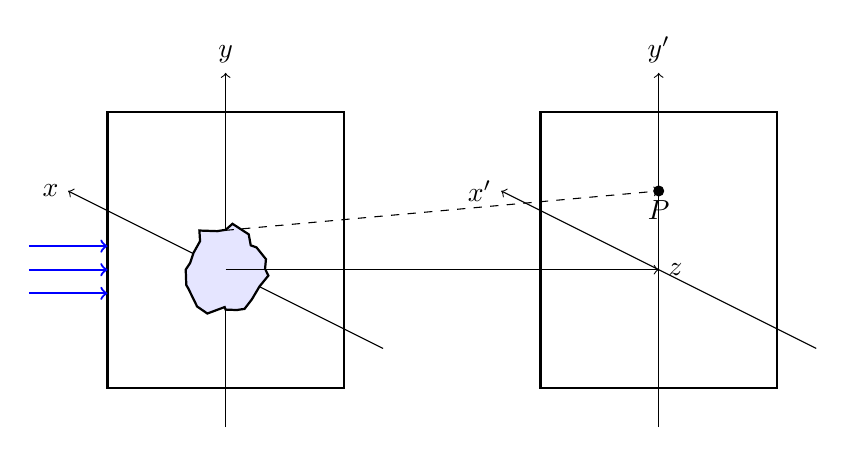
\begin{tikzpicture}
		% Плоскость 1 (отверстие)
		\draw[thick] (-2, -1.5) rectangle (1, 2);
		\draw[->] (-0.5, -2) -- (-0.5, 2.5) node[above] {$y$};
		\draw[->] (1.5, -1) -- (-2.5, 1) node[left] {$x$};
		
		\draw[thick, fill=blue!10, decorate, decoration={random steps,segment length=4pt,amplitude=2pt}] (-0.5, 0) circle (0.5);
		
		\draw[->, thick, blue] (-3, 0) -- (-2, 0);
		\draw[->, thick, blue] (-3, 0.3) -- (-2, 0.3);
		\draw[->, thick, blue] (-3, -0.3) -- (-2, -0.3);
		
		% Плоскость 2 (экран)
		\begin{scope}[xshift=5cm]
			\draw[thick] (-1.5, -1.5) rectangle (1.5, 2);
			\draw[->] (0, -2) -- (0, 2.5) node[above] {$y'$};
			\draw[->] (2, -1) -- (-2, 1) node[left] {$x'$};
			\fill (0, 1) circle (2pt) node[below] {$P$};
		\end{scope}
		
		\draw[->] (-0.5, 0) -- (5, 0) node[right] {$z$};
		\draw[->, dashed] (-0.5, 0.5) -- (5, 1);
	\end{tikzpicture}
\end{figure}

Так как наблюдение ведется далеко: $K(\alpha) \sim \cos \alpha_0 + \cos \alpha_1 \sim 2$ (поскольку $\alpha_0 = 0$, $\alpha_1 \to 0$).

$$E(x',y',z) \sim \iint dx dy \underbrace{E_0 t(x,y)}_{E'} \frac{e^{ikr}}{r} K(\alpha) \sim \frac{2 E_0}{\lambda} \iint dx dy \, t(x,y) e^{ikr}$$